\documentclass[a4paper,12pt]{article}
\usepackage[spanish]{babel}
\usepackage[utf8]{inputenc}
\usepackage{graphicx}%Inclusión de gráficos
\usepackage{float}%Figuras flotantes
\usepackage[letterpaper,top=1.5cm,bottom=1.5cm,left=1.5cm,right=1.5cm]{geometry}
\usepackage{amsfonts}
\usepackage{amssymb}
\usepackage{afterpage}%Para páginas en blanco
\usepackage{hyperref}%Índice dinámico
\sloppy
\begin{document}
\begin{titlepage}\sloppy
\begin{center}
\vspace{2cm}
\begin{figure}[htb]
\begin{center}

\includegraphics[width=4cm]{UNAM.jpeg}
\end{center}
\end{figure}
UNIVERSIDAD NACIONAL AUTÓNOMA DE MÉXICO\\
FACULTAD DE ESTUDIOS SUPERIORES ACATLÁN\\
\vspace{0.15in}
Matemáticas Aplicadas y Computación\\
\vspace{0.6cm}
\vspace{0.6cm}
\begin{Large}
\textbf{} \\
\end{Large}
\vspace{0.3cm}
\begin{large}
\textbf{\Huge{Minería de Datos en el análisis de predicción en bienes raíces}}\\
\end{large}
\vspace{0.3cm}
\rule{80mm}{0.1mm}\\
\vspace{0.1in}
Integrantes:\\
\vspace{2cm}
Antonio Rojas Alexis David\\
\vspace{0.1cm}
Galván Sandoval Diego Alexis\\
\vspace{0.1cm}
Garzón Hernández José Emmanuel\\
\vspace{0.1cm}
Valtierra Iparrea Daniel\\
\vspace{0.1cm}
Vázquez Montoya Víctor Hugo.\\
\vspace{2cm}
\begin{large}
Grupo: 2801
\end{large}
\end{center}
\end{titlepage}
%\pagestyle{empty}
\tableofcontents
%\newpage
\section{Resumen Ejecutivo}
Existe una gran variedad de metodologías de predicción que han sido aplicadas exitosamente en los mercados de negocios tales como 
las acciones, los bonos, etc. El objetivo de este estudio es predecir el precio de los bienes raíces de una empresa líder en el 
mercado durante los últimos años en México, particularmente en la zona metropolitana, en la Ciudad de México, dicha empresa es 
conocida bajo su nombre comercial \textit{Properaty}. Es un nuevo portal web de propiedades que busca mejorar la 
experiencia de compra, venta y alquiler de inmuebles en Argentina. Properati proviene del Latin ``Properatus'' que significa 
``moverse de una forma rápida'' lo cual refleja la idea de un sitio ágil que le permita al usuario encontrar rápidamente su 
futura propiedad\cite{url}. Para dicha predicción será necesario hacer previamente un analisis preeliminar de la información que 
se tenga presente; los datos correspondientes a dos conjuntos principales: el de rentas y ventas respectivamente. La importancia 
de hacer el presente estudio es para hallar modelos que puedan ser predictivos para llegar a la fase final del sistema de 
información, es decir, donde se tenga conocimiento y aqui mismo tomar una decisión importante para un esquema de negocios.
\section{Planteamiento del problema}
La problemática a manejar dentro del presente estudio surge de la necesidad de que no se conoce un buen modelo hasta el momento 
que pueda predecir precios en los distintos puntos del país, especificando las rentas y ventas de los bienes raíces para una mayor 
agilidad en la toma de decisiones.
\section{Objetivos}
\subsection{Objetivo General}
\textit{Encontrar regiones en la zona metropolitana, las cuales sean de oportunidad para las constructoras. Además de darle un 
enfoque de negocios para la constructora también se pretende dar una predicción mediante un tablero dinámico a los clientes para 
que ellos puedan saber qué lugares son más económicos, cuáles son más espaciosos, etc.}
\subsection{Objetivo Particular}
Indicar cómo se están comportando los precios en diferentes etapas de las acciones de negocio por parte de las constructores 
basándose en los parámetros obtenidos del buen modelado que se haya aplicado, como meta se pretende hallar patrones que den como 
resultado un ajuste para entrenar dichos modelos, lo cual nos indicaría  dónde están los lugares, casas, departamentos  más 
rentados o vendidos del México.
\section{Marco Teórico}%%Aqui va todo lo relacionado a los papers.
Estudios recientes sobre el uso de los algoritmos aprendizaje máquina para predecir precios, se han basado en el caso de las 
ventas de casas durante el año 2015 en los precios que determina la Standar \& Poor's, una empresa financiera estadounidense, la 
cual publica informes sobre investigación financiera y análisis de acciones  y bonos.\\
\vspace{3mm}

De acuerdo con lo trabajado por \cite{park2015using} hace un caso del condado de Faifax, en el estado de Virginia. Los datos 
utilizados son de vivienda en general, dichos datos presentan tendencias de mercado en la parte inmobiliaria, el desarrollo del 
esestudio se basa como parte  en la predicción de los precios futuros de la vivienda hasta incluso el establecimiento de 
políticas inmobiliarias. Su metodología se centra en el uso de algoritmos de aprendizaje máquina como se venía recordando para 
desarrollar un modelo de predicción de precios de vivienda. Haciendo una precisión que en el presente documento se hará lo mismo 
pero con un análisis más detallado y exhaustivo con distintos modelos.
\vspace{5mm}

Recalcando el hecho de que las decisiones que se toman con los modelos, se deben ajustar a uno solo donde se encuentre el mejor 
ajuste a aquel modelo ya sea mediante la mejor área bajo la curva ROC por ejemplo, un modelo de árboles de decisión y que el 
método de los pesos evidentes (WOE) ayude a redimensinar el modelo haga los cortes para redimensionar con las variables del 
conjunto de datos y que haga como lo indica su nombre, que sea un buen clasificador en la toma de decisiones.
\vspace{5mm}

Desde una perspectiva metodológica, los modelos existentes de previsión de precios en el Hous-dominio del mercado podría dividirse 
en modelos basados en la teoría y modelos basados en datos. Extensas exploraciones de preguntas que
están asociados con la previsión de direcciones del mercado se han esforzado, incluyendo Dónde está el giro punto de la vivienda 
variaciones de precios
\vspace{5mm}

Dentro de lo que se analiza en \cite{cortes1995support} es la determinación de un umbral en la red neuronal (NN) que sea óptimo 
para las probabilidad de clase y los costos de clasificación, también es importante tener la obtención de estimaciones calibradas 
de  las probabilidades posteriores (a futuro). Para clasificadores binarios un valor límite se controla cómo las probabilidades 
posteriores predichas se convierten en etiquetas de clase. El objetivo de las curvas ROC y otros gráficas es servir de utilidad  
para poder visualizar y analizar la relación entre una o dos medidas de rendimiento.\\
\vspace{5mm}

Para los modelos de predicción de precio, en \cite{park2015using} se hace una valuación del precio, dicha valuación no se hace en 
el trabajo presente ya que dentro de los dos conjuntos de datos se manejan precios de al menos \textit{tres} distintas monedas. 
Regresando al análisis, se hallaron dos principales tendencias: el uso del enfoque de  regresión basado en tecnología de 
inteligencia artificial, y el desarrollo de modelos de predicción de precios de vivienda. Una vez estimado el modelo de regresión 
semi-paramétrica y se comparó la predicción de precios a diferencia  de los modelos paramétricos convencionales, con lo que 
reveló la medición y predicción de las ventas y rentas de casas.
\vspace{5mm}

Las instituciones financieras intentan obtener una estimación precisa del valor del mercado para gestionar mejor el riesgo y por 
consiguiente reduzca el costo relacionado relacionado con la financiación de la vivienda, además, hay muchas cuidades y condados 
basan los impuestos  sobre la propuedad en el valor de mercado de una casa, el cual debe ser actualizado peridódicamente. La 
evaluación inexacta de los valores de la vivienda pueden dar lugar a ajustes substanciales del impuesto sobre la propiedad. Sin 
embargo, la predicción exacta del precio de la casa es difícil porque una vivienda residencial, por ejemplo, es un bien compuesto 
que es vendido típicamente como paquete de varios factores, tales como\textit{localización, ambiente, zona, etc.}. Dado un 
conjunto de atributos de vivienda, lo que se recomienda hacer primero es el de análisis de regresión de los modelos de 
precios\cite{bin2004prediction}.
\vspace{5mm}

La propuesta de modelos actualmente tiene un auge muy amplio en el sentido de hacer previsiones de dinámicas especiales en el 
mercado inmobiliario, pues estudios recientes  como \cite{chen2017forecasting} señalan que el hecho de usar Máquinas Vector 
Soporte, de su equivalente en inglés: \textit{Support Vector Machine (SVM)}. Su marco analítico consta de dos pasos: 
\textit{identificación de los vectores de apoyo a las varianzas de precios mediante la regresión gradial} y luego \textit{es 
pronosticar ñas variaciones de precios de la vivienda empleando a la máquina vector soporte identificada}. Los resultados 
utlizados por dichos investigadores cnfirman que la estimación paramétrica es poco sugerida en el entrenamiento de este tipo de 
modelos y que el poder de predicción de una SVM tiene más alta precisión paa extraer información geográficos utilizando el kernel 
dond elas estimaciones de densidad para reflejar respuestas de precio a cuantiles. locales de ciertos atributos en el conjunto 
de datos. 
\section{Análisis Exploratorio de Datos}
El Análisis Exploratorio de Datos es quien tiene como objetivo identificar el comportamiento matemático o la forma matemática en 
la que se encuentra actualmente la BD y así orientar al analista a poder comprender mejor cómo trabajar con ellos. La dos bases de 
datos obtenidas, describen cada una por su cuenta los precios, área en metros cuadrados, ubicación geográfica entre otros datos ya 
sea el caso analizado, para rentas o ventas de bienes raíces como anteriormente ya se ha señalado.\\
Los datos de la base de rentas tienen un total de 47147 tuplas, distribuidos en 27 atributos de las cuales algunas muestran datos 
irrelevantes para modelar, puesto que solo son indicadores de informacion adicional para fines del negocio .Las variables son 
analizadas ampliamente ya que en algunos casos no se cuenta con información suficiente en los atributos que pueda proporcionar 
relevancia (missings) y por lo tanto pueden causar un error en el modelo analitico que se busca realizar.
Las columnas de la base de datos de rentas, que se considerarán para el análisis son:
\vspace{5mm}

\begin{itemize}
\item Created on: Fecha de creación del archivo para la renta de ese propiedad.
\item Place name: Nombre del lugar en donde esta en renta la propiedad.
\item Country name: Nombre de la ciudad donde está la propiedad.
\item Lat: Latitud geográfica.
\item Lon: Longitud geográfica.
\item Price: Precio de la renta de la propiedad.
\item Currency: Moneda con la que se trabaja el precio de la renta ['USD', 'ARS', 'MXN'].
\item Surface total in m2: Área total en metros cuadrados de la propiedad.
\item Price per $m^2$: Precio por metro cuadrado de la propiedad, considerada en ['USD', 'ARS', 'MXN'].
\item Rooms: Número de habitaciones en la propiedad.
\end{itemize}

Los datos de cada atributo permiten poder observar el comportamiento puesto que hay un parámetro que determina el inicio, 
que es la fecha en que se crea el archivo, el cual permite al analizar los datos, saber un comportamiento de la demanda 
de residencia en cierta ciudad o área determinada geográficamente, con esos datos iniciales los precios que se manejan en las 
distintas zonas nos darán un enfoque para identificar un necesidad de crecimiento urbano en el país. Como los precios que se 
manejan la divisa son los dólares y en pesos se considera una transformación de valores con respecto a la moneda del país (México) 
y con ello manejar todo en una sola divisa.
\vspace{5mm}

Los datos de área total y por metro cuadrado, más los precios de esos mismo parámetros nos permiten ubicar con más exactitud si la 
demanda de rentas son para grandes áreas o pequeñas áreas, indicando así un patrón de precios y áreas específicas en las distntas 
ciudades del país.
\section{Desarrollo}
\subsection{Estructura OLTP}
A continuación se muestra la estructura OLTP en la figura \ref{fig:1}:
\begin{figure}[H]
\begin{center}
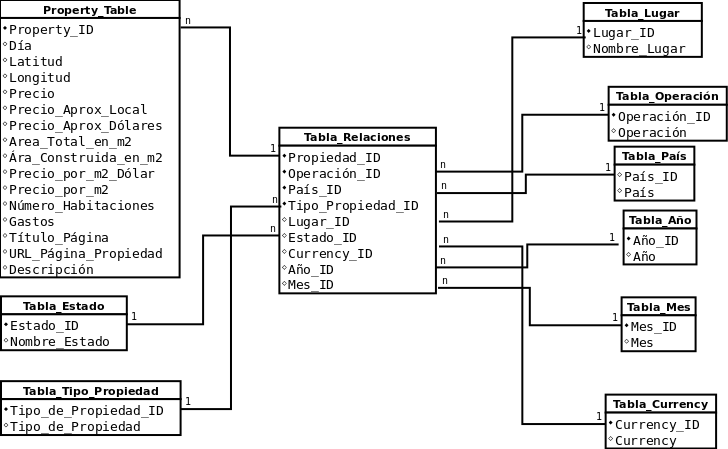
\includegraphics[width=0.35\textwidth]{OLTP_2904_PRO.png}
\caption{OnLine Transactional Process}\label{fig:1}
\end{center} 
\end{figure}
\subsection{Estructura OLAP}
Como se puede apreciar en la figura \ref{fig:2} la estructura OLAP presentada a continuación:
\begin{figure}[H]
\begin{center}
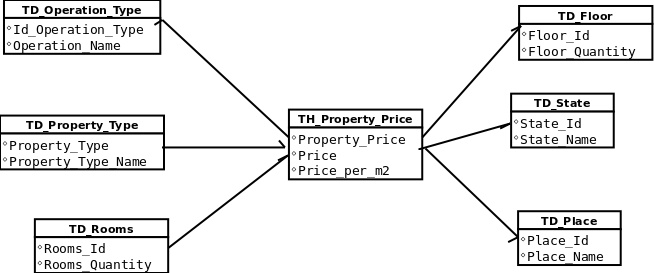
\includegraphics[width=0.50\textwidth]{OLAP.png}
\caption{On Line Analytical Proccesing}\label{fig:2}
\end{center}
\end{figure}
\section{Modelo Supervisado}
\section{Modelo No Supervisado}
\section{Bibliografía}
\bibliographystyle{apalike}
%\renewcommand{\bibname}{Referencias}
\bibliography{Refere}
\nocite{*}
\end{document}